Various parts of the implementation were created with extensibility in mind and are structured in such a way that the constraint validation engine is decoupled from the visualization part (see Figure \ref{fig:structure_of_the_implementation}). This makes the individual components easily maintainable and extensions to the implementation can be made with ease. Further, it turns out that the constraint validation engine is agnostic to the SHACL engine and the machine learning model used.  

\paragraph{Constraints} 
\begin{figure}
    \centering
    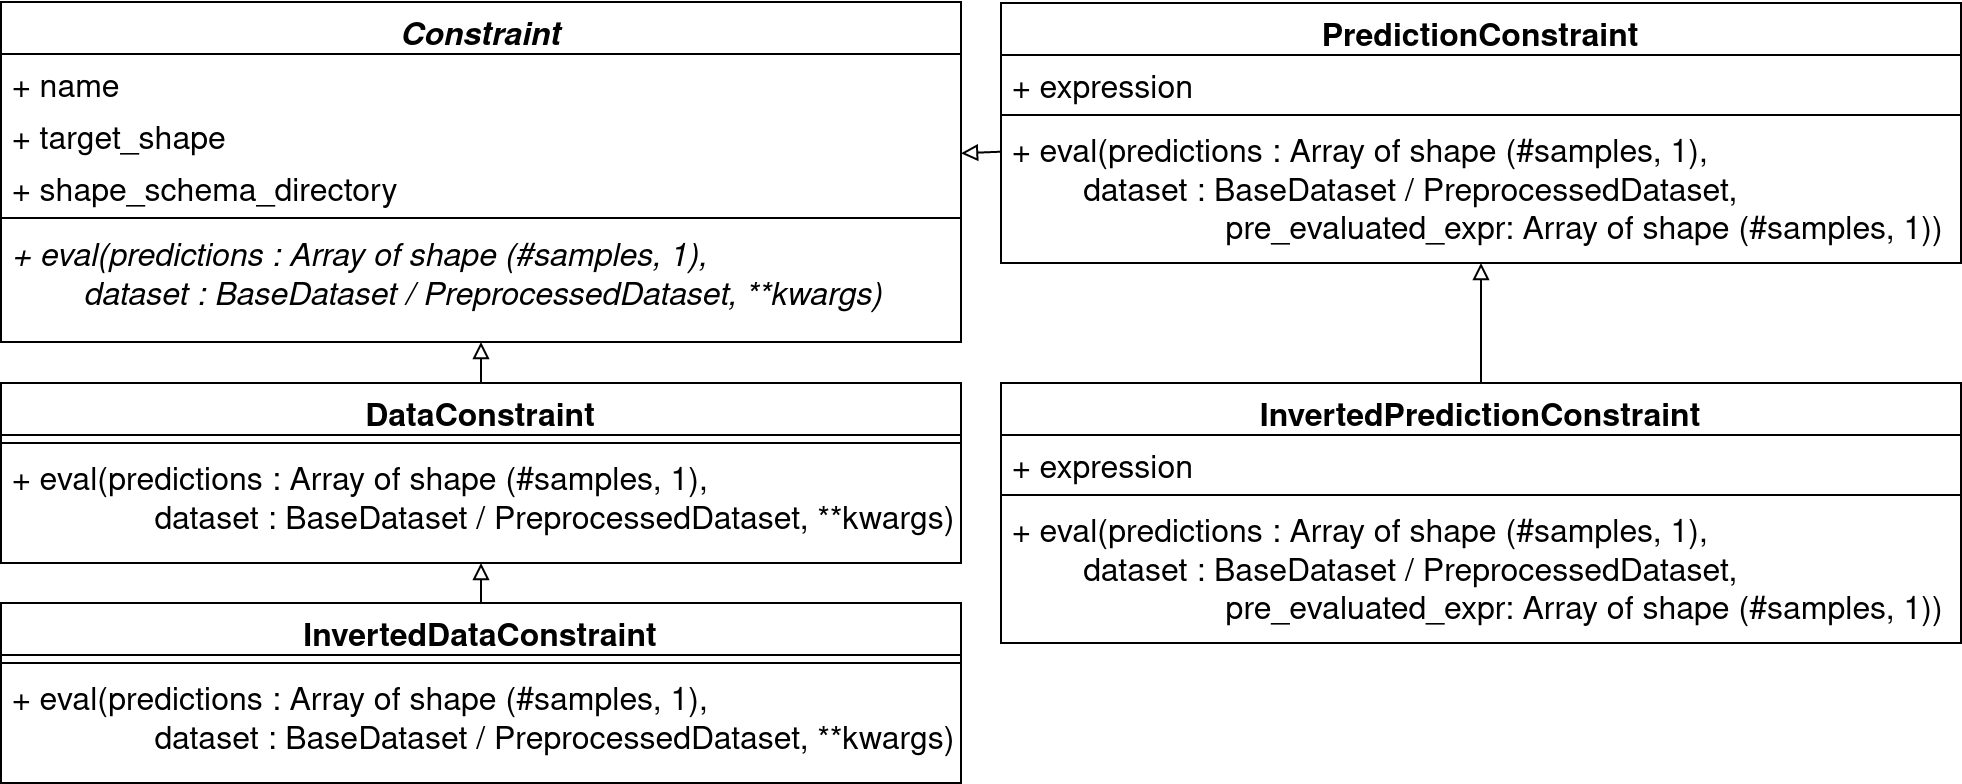
\includegraphics[width=\textwidth]{images/implementation/Constraint.png}
    \caption{The \textsc{Constraint} Module}
    \label{fig:the_constraint_module}
\end{figure}
The \textsc{Constraint} module (see Figure \ref{fig:the_constraint_module}) provides implementations of the constraint types described in section \ref{section_further_types_of_constraints}. A central concept is the usage of SHACL constraints to make use of the semantic context of the entities in the knowledge graph which are connected to the samples in the dataset. Therefore, the abstract base class \emph{Constraint} provides the capabilities to integrate SHACL validation results into the constraint evaluation. All constraint types have to inherit from \emph{Constraint} and implement the ``eval'' method, to be usable with the constraint validation engine. As an example, the \emph{PredictionConstraint} class implements the type of constraint defined in definition \ref{Def:constraint} by extending \emph{Constraint} with an expression representing the right-hand side of the prediction constraint. A user may change the semantics of the prediction or data constraint by inheriting from them. As an example, the implementation provides inverted constraints, which invert the constraint validation result.



\paragraph{SHACL Engines} 
\begin{figure}
    \centering
    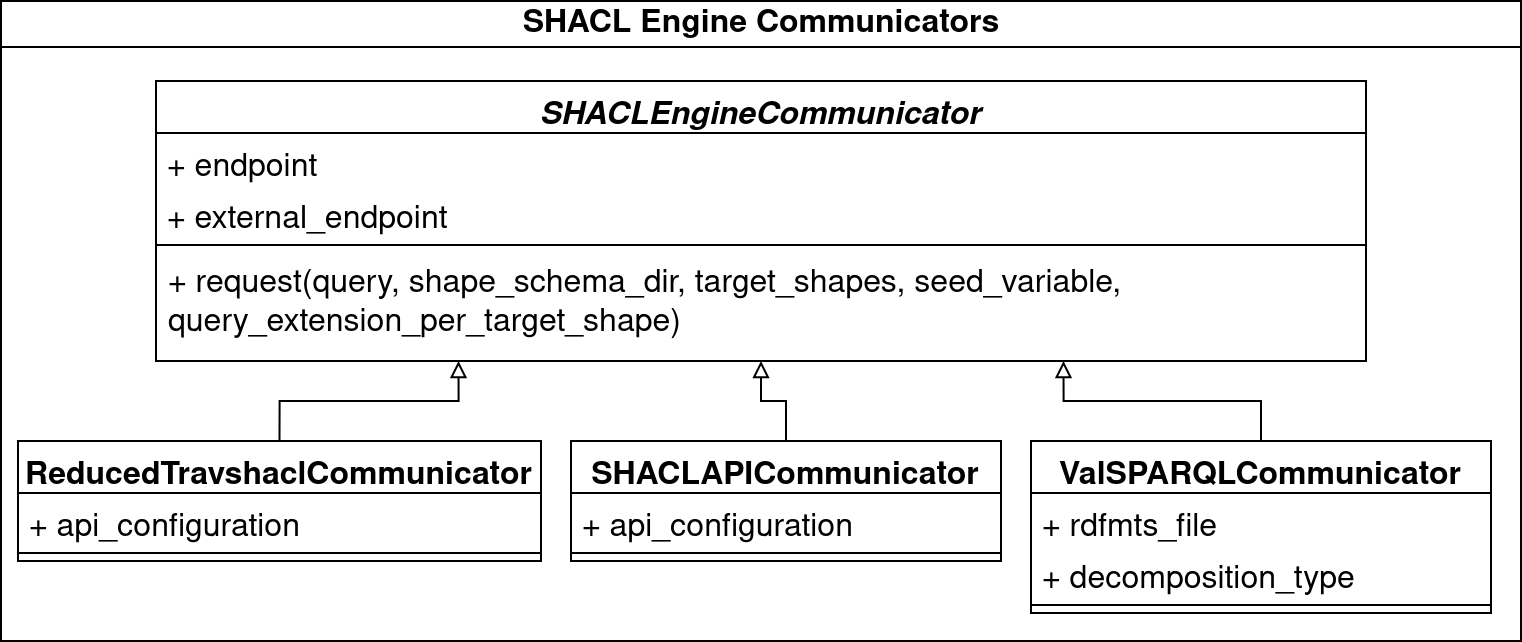
\includegraphics[width=0.8\textwidth]{images/implementation/shacl_engines_communicator.png}
    \caption{The SHACL Engines Communicator Module}
    \label{fig:shacl_engines_module}
\end{figure}
The \textsc{SHACL Engines Communicator} module (see Figure \ref{fig:shacl_engines_module}) makes the constraint validation engine agnostic to the SHACL engine used. A communicator to be used by the \textsc{Dataset} module has to inherit from the abstract base class \emph{SHACLEngineCommunicator} and has two endpoints assigned. The first one corresponds to an internal endpoint like the shaclAPI (Figure \ref{fig:shacl_api}) and the second one is an external link to the SPARQL endpoint used as the data source and for SHACL validation. Three different communicators are already implemented: The \emph{ReducedTravshaclCommunicator} directly integrates the shaclAPI to reduce the SHACL shape schema for Trav-SHACL \cite{figuera2021trav}. The second and the third ones implement the concept of performing the SHACL constraint validation during SPARQL query execution as described in section \ref{section_valSPARQL}. The \emph{SHACLAPICommunicator} makes use of extended capabilities of the shaclAPI to join SPARQL query results with SHACL validation results, while the \emph{ValSPARQLCommunicator} uses the valSPARQL engine to push down the join into the SPARQL query evaluation.

\paragraph{Checker} The \textsc{Checker} module includes the \emph{Checker} class as depicted in Figure \ref{fig:checker_implementation} and is model-implementation-agnostic as only one function is required to get predictions from the model. For instance, the implementation of example \ref{Bsp:node_based_constraint_validation} does not require to make any changes to the \emph{Checker} class. Although, the predictions are now based on the decision tree node and not the whole decision tree. Instead, a prediction method can be defined to return the constant predictions, which would be made by the node (see section \ref{section_tree_based_models}). 

\paragraph{Group Functions} 
\begin{figure}
    \centering
    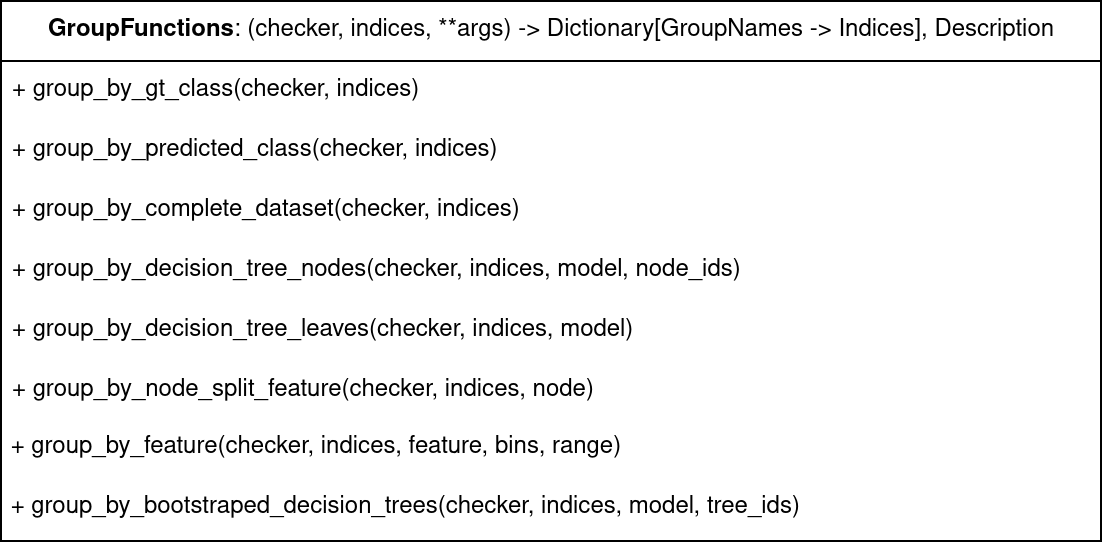
\includegraphics[width=0.8\textwidth]{images/implementation/group_functions.png}
    \caption{The \textsc{Group Functions} Module}
    \label{fig:the_group_functions_module}
\end{figure}
Group functions are a concept introduced in definition \ref{Def:frequency_distribution_creation_function}. Formally, they take a group name and return a set of indices of samples from the dataset belonging to that group. In the implementation, a group function in the \textsc{Group Functions} module (see Figure \ref{fig:the_group_functions_module}) takes an instance of the \emph{Checker} class and the indices of the dataset to be grouped and returns a dictionary mapping each of the group names to the subset of indices belonging to that group and a description string saying how the grouping is named. The checker instance provides all the components (e.g., the problem instances, the targets, the predictions, and the sample-to-node mapping) which might be needed to group the indices. However, further arguments might be provided to the group functions if needed. For example, the ``group\_by\_feature'' function; generating the theoretical $\Gamma_\text{bins}^{f_k}$ function, additional takes the feature, the number of bins, and the range for the binning as inputs. Therefore, new grouping functions can be added easily and used in existing visualizations. For instance, the visualization of the leaves in the decision tree makes use of a grouping function to determine the frequency distribution to show (e.g., Figure \ref{fig:multiple_constraints_gt_annotated_motivating_example_decision_tree} makes use of group\_by\_gt ($\Gamma_\text{gt}$) and Figure \ref{fig:multiple_constraints_per_node_annotated_motivating_example_decision_tree} makes use of group\_by\_complete\_dataset ($\Gamma_\text{all}$)).

\paragraph{Visualizations}
\begin{figure}
    \centering
    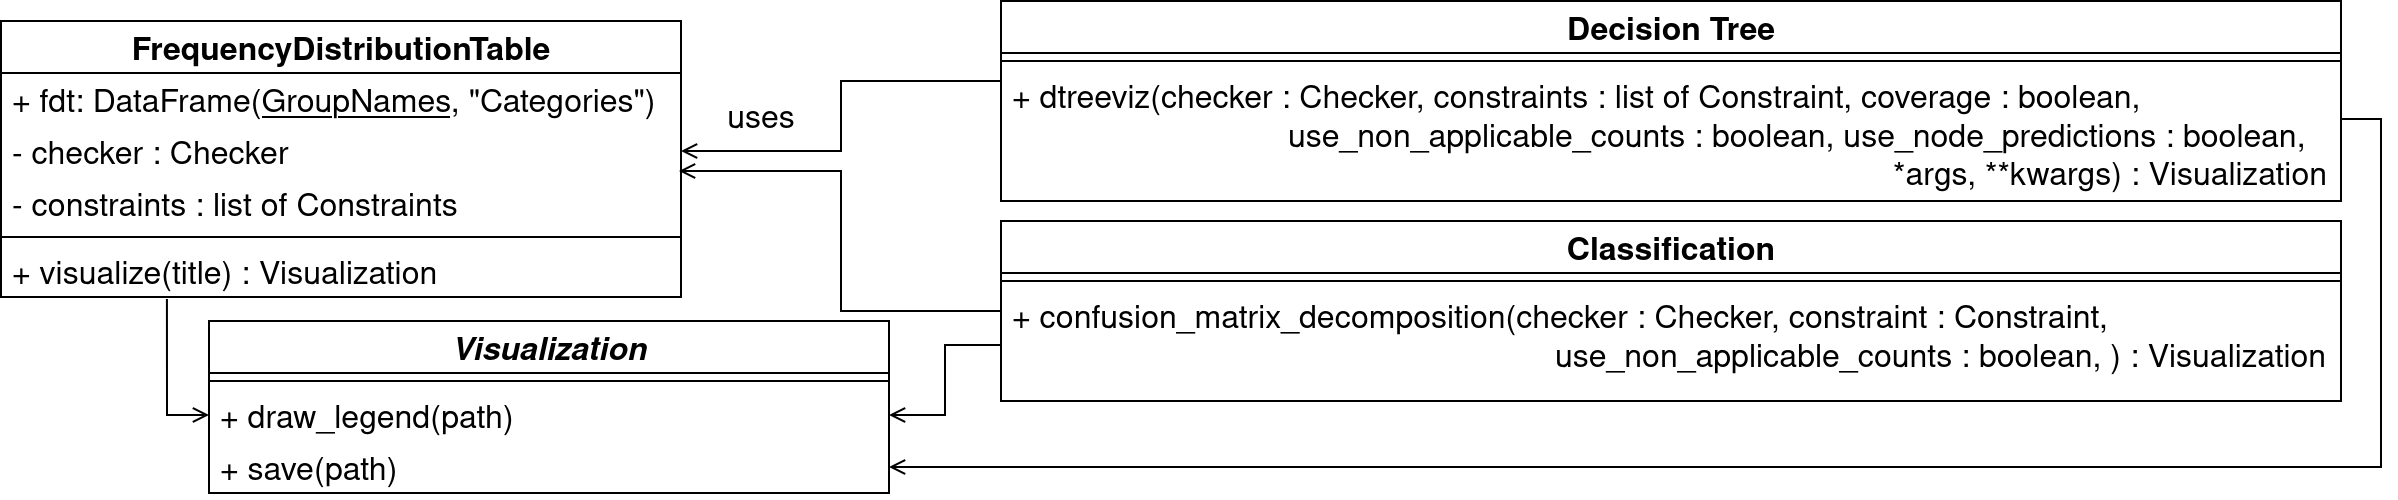
\includegraphics[width=\textwidth]{images/implementation/Visualization.png}
    \caption{The \textsc{Visualization} Module}
    \label{fig:the_visualization_module}
\end{figure}
In general, the visualizations generated are specific to the model. However, frequency distributions and the according visualizations can be used independently of the model. That is the concepts shown in sections \ref{section_frequency_distribution_tables} and \ref{section_visualizing_multiple_constraint_validation_results} can be applied independent of the chosen model. The information content and the connection to the internal structure of the model then depend only on the grouping function and the fraction of the samples in the dataset selected to be visualized at once. Therefore, the work done in sections \ref{section_constraint_decision_tree_visualization} and \ref{section_confusion_matrix_decomposition} is an example of a suitable composition of frequency distributions which can be created for other models as well. Figure \ref{fig:the_visualization_module} shows roughly the content of the \textsc{Visualization} module. 


\paragraph{Shadow Model}
The visualization of the model w.r.t. the constraints is based on the internals of the model. However, the library can be chosen according to the user's preference as the visualization algorithm is independent of the concrete implementation of the model, but instead makes use of the adapter pattern (reused from the dtreeviz library \cite{dtreeviz}; see Figure \ref{fig:adapterPatternShadowModels}).



%The python implementation comes with a documentation\footnote{\href{https://julianloewe.github.io/Validating_Models/}{https://julianloewe.github.io/Validating\_Models/}}



% --> SHACL Engine Communicators -> Abstract Base Class to extend. The implementation is not bound to a specifc engine --> Showing the Engine Package => Available backends

% --> New Types of Constraints can be added --> Showing the Constraint Package

% --> The Checker instances also allows to be extended --> Example Node Checker, New Group Functions

% --> The libraries used to get the internal information about the model can be swapped, as the implementation relies on the ShadowModel introduced by the dtreeviz library.








